% Template for solutions write-ups, STAT 460/560
% Some basic notation is defined in 'macros/basic-math-macros'

\documentclass{article}
\usepackage{verbatim}
\usepackage{titlesec}

\def\coursename{STAT 447C: Bayesian Statistics}
\def\semester{Fall 2024}

\setlength{\oddsidemargin}{0.0 in}
\setlength{\evensidemargin}{0.0 in} 
\setlength{\topmargin}{-0.6 in} 
\setlength{\textwidth}{6.5 in} 
\setlength{\textheight}{8.5 in}
\setlength{\headsep}{0.75 in} 
\setlength{\parindent}{0 in}
\setlength{\parskip}{0.1 in}

\titleformat*{\section}{\Large\bfseries}


% prints box at top of first page with relevant info
\newcommand{\problemset}[3]{
   \pagestyle{myheadings}
   \thispagestyle{plain}
   \newpage
   \noindent
   \begin{center}
   \framebox{
      \vbox{\vspace{2mm}
    \hbox to 6.28in { {\bf \coursename
                        \hfill \semester} }
       \vspace{4mm}
       \hbox to 6.28in { {\Large \hfill #3  \hfill} }
       \vspace{2mm}
       \hbox to 6.28in { {\it #1 \hfill \texttt{#2}} }
      \vspace{2mm}}
   }
   \end{center}
   \vspace*{4mm}
}

\newcommand{\qsol}[1]{\section{#1}}
  % DO NOT CHANGE
% \usepackage{graphicx,amssymb,amsmath,amsthm,mathrsfs}
% \usepackage{multirow,makeidx,algorithmic,algorithm}
\usepackage{multirow,makeidx,algpseudocode,algorithm}
\usepackage{mathtools}
\usepackage{enumitem}
 
\usepackage{parskip}
\usepackage{setspace}
\usepackage{float, graphicx}
\usepackage{adjustbox}
\usepackage{bbm}
\usepackage{tabularx}
\usepackage{subfigure}
\usepackage{amsmath,amssymb,amsfonts,amsthm,amsbsy,amstext,mathrsfs}
\usepackage{hyperref}
\usepackage{url}
\usepackage{color}
\usepackage{graphicx} % Required for inserting images
\usepackage[utf8]{inputenc}

%% reference
\usepackage[round]{natbib}
\bibliographystyle{abbrvnat}
% \usepackage{cite}
% \bibliographystyle{plainurl}
% \bibliographystyle{abbrv}
% \bibliographystyle{plain}
% \bibliographystyle{unsrt}


%% code in-text
\usepackage{listings}
\usepackage{xcolor}

\definecolor{codegreen}{rgb}{0,0.6,0}
\definecolor{codegray}{rgb}{0.5,0.5,0.5}
\definecolor{codepurple}{rgb}{0.58,0,0.82}
\definecolor{backcolour}{rgb}{0.95,0.95,0.92}

\lstdefinestyle{mystyle}{
    backgroundcolor=\color{backcolour},   
    commentstyle=\color{codegreen},
    keywordstyle=\color{magenta},
    numberstyle=\tiny\color{codegray},
    stringstyle=\color{codepurple},
    basicstyle=\ttfamily\footnotesize,
    breakatwhitespace=false,         
    breaklines=true,                 
    captionpos=b,                    
    keepspaces=true,                 
    numbers=left,                    
    numbersep=5pt,                  
    showspaces=false,                
    showstringspaces=false,
    showtabs=false,                  
    tabsize=2
}

\lstset{style=mystyle}


%% layout
\oddsidemargin 3mm
\evensidemargin 3mm
\topmargin -12mm
\textheight 660pt
\textwidth 450pt  % DO NOT CHANGE
% ADD YOUR CUSTOM NOTATION HERE
\newcommand{\R}{\mathbb R}
\newcommand{\Z}{\mathbb Z}
\newcommand{\Q}{\mathbb Q}
\newcommand{\N}{\mathbb N}
\newcommand{\C}{\mathbb{C}}
\newcommand{\1}{\mathbbm{1}}
\newcommand{\E}{\mathbb E}
\newcommand{\Mcal}{{\cal M}}
\newcommand{\Ncal}{{\cal N}}
\newcommand{\Acal}{{\cal A}}
\newcommand{\Bcal}{{\cal B}}
\newcommand{\Fcal}{{\cal F}}
\newcommand{\Ecal}{{\cal E}}
\newcommand{\Gcal}{{\cal G}}
\newcommand{\Hcal}{{\cal H}}
\newcommand{\Scal}{{\cal S}}
\newcommand{\Xcal}{{\cal X}}
\newcommand{\Lcal}{{\cal L}}
\newcommand{\Mscr}{\mathscr{M}}
\newcommand{\eps}{\varepsilon}
\renewcommand{\P}{\mathbb P}
\DeclareMathOperator{\Var}{Var}
\DeclareMathOperator{\Poi}{Poi}
\DeclareMathOperator{\Cov}{Cov}
\DeclareMathOperator{\Exp}{Exp}
\DeclareMathOperator{\Bin}{Bin}
\DeclareMathOperator{\Geom}{Geom}
\DeclareMathOperator{\Unif}{Unif}
\DeclareMathOperator{\Bernoulli}{Bernoulli}
\DeclareMathOperator{\BetaMP}{BetaMP}
\DeclareMathOperator{\Beta}{Beta}
\newcommand{\abs}[1]{\left|#1\right|}
\newcommand{\norm}[1]{\left\lVert#1\right\rVert}
\newcommand{\floor}[1]{\lfloor#1\rfloor}
\newcommand{\ceil}[1]{\lceil#1\rceil}
\newcommand{\ds}{\displaystyle}
\newcommand{\inv}[1]{#1^{-1}}
\newcommand{\vect}[1]{\boldsymbol{#1}}
\DeclareMathOperator*{\argmax}{arg\,max}
\DeclareMathOperator*{\argmin}{arg\,min}
\newcommand{\convdist}[0]{\overset{d}{\longrightarrow}}
\newcommand{\convprob}[0]{\overset{p}{\longrightarrow}}
\newcommand{\convas}[0]{\overset{a.s.}{\longrightarrow}}
\newcommand{\partiald}[1]{\frac{\partial}{\partial{#1}}}
\newcommand{\partialdd}[1]{\frac{\partial^2}{\partial{#1^2}}}
% \newtheorem{definition}{Definition}[section]
% \newtheorem{theorem}{Theorem}[section]
% \newtheorem{corollary}{Corollary}[theorem]
% \newtheorem{lemma}{Lemma}[theorem]
% \newtheorem{proposition}[theorem]{Proposition}

\newtheorem{definition}{Definition}[section]
\newtheorem{theorem}{Theorem}[section]
\newtheorem{corollary}{Corollary}[section]
\newtheorem{lemma}{Lemma}[section]
\newtheorem{proposition}{Proposition}[section]
\newtheorem*{remark}{Remark}

\renewcommand{\algorithmicrequire}{ \textbf{Input:}} %Use Input in the format of Algorithm
\renewcommand{\algorithmicensure}{ \textbf{Output:}} %UseOutput in the format of Algorithm


%%
% full alphabets of different styles
%%

% bf series
\def\bfA{\mathbf{A}}
\def\bfB{\mathbf{B}}
\def\bfC{\mathbf{C}}
\def\bfD{\mathbf{D}}
\def\bfE{\mathbf{E}}
\def\bfF{\mathbf{F}}
\def\bfG{\mathbf{G}}
\def\bfH{\mathbf{H}}
\def\bfI{\mathbf{I}}
\def\bfJ{\mathbf{J}}
\def\bfK{\mathbf{K}}
\def\bfL{\mathbf{L}}
\def\bfM{\mathbf{M}}
\def\bfN{\mathbf{N}}
\def\bfO{\mathbf{O}}
\def\bfP{\mathbf{P}}
\def\bfQ{\mathbf{Q}}
\def\bfR{\mathbf{R}}
\def\bfS{\mathbf{S}}
\def\bfT{\mathbf{T}}
\def\bfU{\mathbf{U}}
\def\bfV{\mathbf{V}}
\def\bfW{\mathbf{W}}
\def\bfX{\mathbf{X}}
\def\bfY{\mathbf{Y}}
\def\bfZ{\mathbf{Z}}

% bb series
\def\bbA{\mathbb{A}}
\def\bbB{\mathbb{B}}
\def\bbC{\mathbb{C}}
\def\bbD{\mathbb{D}}
\def\bbE{\mathbb{E}}
\def\bbF{\mathbb{F}}
\def\bbG{\mathbb{G}}
\def\bbH{\mathbb{H}}
\def\bbI{\mathbb{I}}
\def\bbJ{\mathbb{J}}
\def\bbK{\mathbb{K}}
\def\bbL{\mathbb{L}}
\def\bbM{\mathbb{M}}
\def\bbN{\mathbb{N}}
\def\bbO{\mathbb{O}}
\def\bbP{\mathbb{P}}
\def\bbQ{\mathbb{Q}}
\def\bbR{\mathbb{R}}
\def\bbS{\mathbb{S}}
\def\bbT{\mathbb{T}}
\def\bbU{\mathbb{U}}
\def\bbV{\mathbb{V}}
\def\bbW{\mathbb{W}}
\def\bbX{\mathbb{X}}
\def\bbY{\mathbb{Y}}
\def\bbZ{\mathbb{Z}}

% cal series
\def\calA{\mathcal{A}}
\def\calB{\mathcal{B}}
\def\calC{\mathcal{C}}
\def\calD{\mathcal{D}}
\def\calE{\mathcal{E}}
\def\calF{\mathcal{F}}
\def\calG{\mathcal{G}}
\def\calH{\mathcal{H}}
\def\calI{\mathcal{I}}
\def\calJ{\mathcal{J}}
\def\calK{\mathcal{K}}
\def\calL{\mathcal{L}}
\def\calM{\mathcal{M}}
\def\calN{\mathcal{N}}
\def\calO{\mathcal{O}}
\def\calP{\mathcal{P}}
\def\calQ{\mathcal{Q}}
\def\calR{\mathcal{R}}
\def\calS{\mathcal{S}}
\def\calT{\mathcal{T}}
\def\calU{\mathcal{U}}
\def\calV{\mathcal{V}}
\def\calW{\mathcal{W}}
\def\calX{\mathcal{X}}
\def\calY{\mathcal{Y}}
\def\calZ{\mathcal{Z}}


%%%%%%%%%%%%%%%%%%%%%%%%%%%%%%%%%%%%%%%%%%%%%%%%%%%%%%%%%%
% text short-cuts
\def\iid{i.i.d.\ } %i.i.d.
\def\ie{i.e.\ }
\def\eg{e.g.\ }
\def\Polya{P\'{o}lya\ }
%%%%%%%%%%%%%%%%%%%%%%%%%%%%%%%%%%%%%%%%%%%%%%%%%%%%%%%%%%

% set theory/measure theory
\def\collection{\calC}
\newcommand{\sigalg}[1]{\mathcal{#1}}
\def\borel{\calB} %Borel sets
\def\sigAlg{\sigalg{H}} %sigma-algebra
\def\filtration{\calF} %filtration
\newcommand{\msblSpace}[1]{(#1,\sigalg{#1})}
\newcommand{\measSpace}[2][\mu]{(#2,\sigalg{#2},#1)}
\newcommand{\borelSpace}[1]{(#1,\borel(#1))}
\newcommand{\measFuncs}[1]{\sigalg{#1}^f}
\newcommand{\pbblSpace}{(\Omega,\sigAlg)}
\newcommand{\probSpace}[1][\bbP]{(\Omega,\sigAlg,#1)}

\def\leb{\lambda}

\def\finv{f^{-1}} % inverse
\def\ginv{g^{-1}} % inverse

% group theory
\def\grp{\calG} %group

% operators
\def\P{\bbP} %fundamental probability
\def\E{\bbE} %expectation
% conditional expectation
\DeclarePairedDelimiterX\bigCond[2]{[}{]}{#1 \;\delimsize\vert\; #2}
\newcommand{\conditional}[3][]{\bbE_{#1}\bigCond*{#2}{#3}}
\def\Law{\mathcal{L}} %law; this is by convention in the literature
% \def\indicator{\mathds{1}} % indicator function
\def\1{{\mathbf 1}}
\def\indicator{\1}

% binary relations
\def\condind{{\perp\!\!\!\perp}} %independence/conditional independence
\def\equdist{\stackrel{\text{\rm\tiny d}}{=}} %equal in distribution
\def\equas{\stackrel{\text{\rm\tiny a.s.}}{=}} %euqal amost surely
\def\simiid{\sim_{\mbox{\tiny iid}}} %sampled i.i.d

% common vectors and matrices
\def\onevec{\mathbf{1}}
\def\iden{\mathbf{I}} % identity matrix
\def\supp{\text{\rm supp}}

% misc
% floor and ceiling
% \DeclarePairedDelimiter{\ceilpair}{\lceil}{\rceil}
% \DeclarePairedDelimiter{\floor}{\lfloor}{\rfloor}
\newcommand{\argdot}{{\,\vcenter{\hbox{\tiny$\bullet$}}\,}} %generic argument dot
%%%%%%%%%%%%%%%%%%%%%%%%%%%%%%%%%%%%%%%%%%%%%%%%%%%%%%%%%%


 
\graphicspath{{./figures/}}







\begin{document}



% FILL IN:
%  - YOUR NAME, YOUR EMAIL (self-explanatory)
%  - The assignment number goes in ##
\problemset{Junsong Tang}{junsong.tang@stat.ubc.ca}{Exercise 5}



% WRITE YOUR SOLUTION TO THE FIRST QUESTION
\qsol{sequential updating} % USE THE SAME TITLES AS ON THE ASSIGNMENT SHEET
\begin{enumerate}
\item 
Denote $\theta | x^{(n)} \sim \pi$. Since $x_i|\theta$ is i.i.d, then $x^{(n)} |\theta \sim v_{\theta}^n$. Suppose $\mu$ is the common dominating measure of $\nu$ and $\rho$, i.e. $p(x_i|\theta) = \frac{d\nu}{d\mu}(x_i)$ and $p(\theta) = \frac{d\rho}{d\mu}(\theta)$, then by Bayes' Theorem, we have:
\[\frac{d\pi}{d\mu}(\theta) = p(\theta | x^{(n)}) = \frac{p(x^{(n)}|\theta) \cdot p(\theta)}{\int_{\Theta} p(x^{(n)}|\theta) \cdot p(\theta) d\mu}\]
Hence\[\pi(d\theta) = \frac{p(x^{(n)}|\theta) \cdot \rho(d\theta)}{\int_{\Theta} p(x^{(n)}|\theta) \cdot \rho(d\theta)} = \frac{\nu_{\theta}^n(dx)\cdot \rho(d\theta)}{\int_{\Theta} \nu_{\theta}^n(dx) \cdot \rho(d\theta)}\]



\item 
Using $\pi$ as the new prior, then by Bayes's Theorem, the posterior distribution of $\theta|x_{n+1}$ is given by:
\begin{align*}
& \frac{p(x_{n+1}|\theta) \cdot \pi(d\theta)}{\int_{\Theta} p(x_{n+1}|\theta) \cdot \pi(d\theta)}\\
& = \frac{\nu_{\theta}(dx_{n+1}) \cdot \nu_{\theta}^n(dx)\cdot \rho(d\theta)}{\int_{\Theta} \nu_{\theta}(dx_{n+1}) \cdot \nu_{\theta}^n(dx)\cdot \rho(d\theta)}\\
& = \frac{\nu_{\theta}^{n+1}(dx) \cdot \rho(d\theta)}{\int_{\Theta} \nu_{\theta}^{n+1}(dx)\cdot \rho(d\theta)}
\end{align*}We can see that is equivalent of using $\rho$ as prior with $(x_1, \ldots, x_{n+1})$ observations.






\end{enumerate}


% WRITE YOUR SOLUTION TO THE SECOND QUESTION
\qsol{Bayesian inference in the limit of increasing data}
\begin{enumerate}
\item 
\begin{lstlisting}[language=R]
# global
library(ggplot2)
suppressPackageStartupMessages(library(extraDistr))
suppressPackageStartupMessages(library(distr))
source("./simple.R")
source("./simple_utils.R")
set.seed(2025)
K = 20

# 1
posterior_distribution = function(rho, n_successes, n_observations) {
  K = length(rho) - 1
  gamma = rho * dbinom(n_successes, n_observations, (0:K)/K)
  normalizing_constant = sum(gamma)
  gamma/normalizing_constant
}
\end{lstlisting}


\item 
\begin{lstlisting}[language=R]
# 2
posterior_mean = function(post_dist) {
    return (sum((seq(0, K, 1)/K) * post_dist))
}
\end{lstlisting}

\item 
\begin{lstlisting}[language=R]
# 3
simulate_posterior_mean_error = function(rho_true, rho_prior, n_observations){
    dist_p = DiscreteDistribution(supp = (1/K)*(0:K), prob = rho_true/sum(rho_true))
    p_true = simulate(dist_p)
    Y = replicate(n_observations, simulate(Bern(p_true)))
    post_dist = posterior_distribution(rho_prior, sum(Y), n_observations)
    post_mean = posterior_mean(post_dist)
    return (abs(p_true - post_mean))
}
\end{lstlisting}

\item 
\begin{lstlisting}[language=R]
# 4
rho_true = rho_prior = 1:(K+1)
n_obs_vector <- 2^(0:6)
experiment_results = data.frame()
for (n_obs in n_obs_vector) {
    errors = replicate(1000, simulate_posterior_mean_error(rho_true, rho_prior, n_obs))
    df = data.frame(n_observations=rep(n_obs, 1000), replication=(1:1000), errors=errors)
    experiment_results = rbind(experiment_results, df)
}
head(experiment_results)
tail(experiment_results)
\end{lstlisting}


\item 
\begin{lstlisting}[language=R]
# 5
ggplot(experiment_results, aes(x=n_observations, y=errors+1e-9)) + # avoid log(0)
    stat_summary(fun = mean, geom="line") + # Line averages over 1000 replicates
    scale_x_log10() +  # Show result in log-log scale
    scale_y_log10(n.breaks=16) +
    coord_cartesian(ylim = c(1e-3, 1)) +
    theme_minimal() +
    geom_point() +
    labs(x = "Number of observations",
        y = "Absolute error of the posterior mean")
\end{lstlisting}
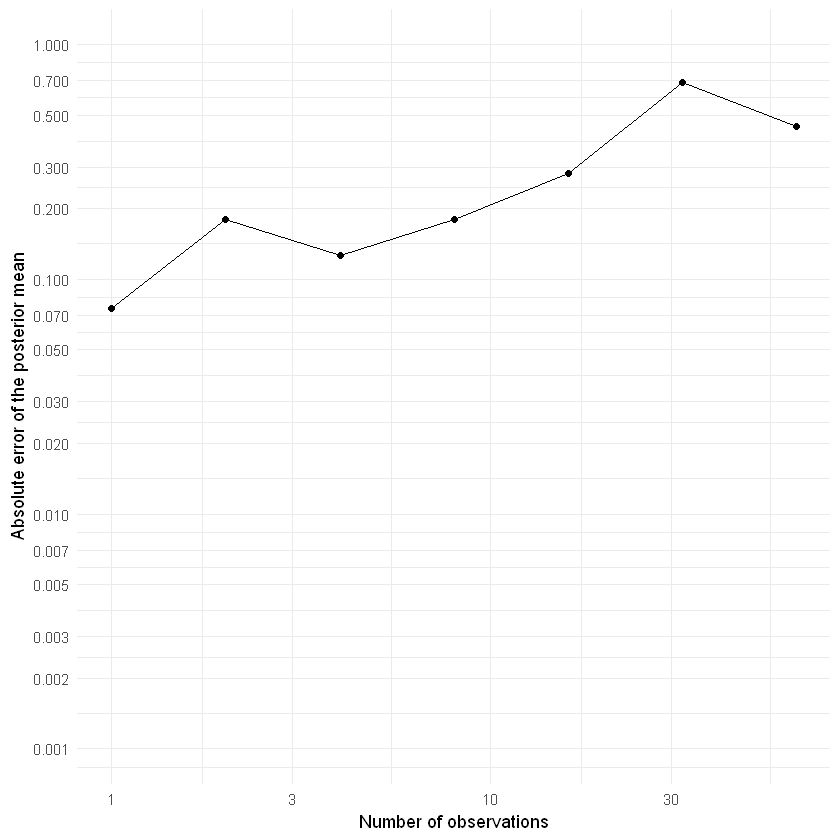
\includegraphics[width=0.8\textwidth]{errors.png}


\item 
\begin{lstlisting}[language=R]
# 6
y7 = mean(experiment_results[experiment_results$n_observations == 2^6, ]$errors)
y5 = mean(experiment_results[experiment_results$n_observations==2^4, ]$errors)
(log10(y7) - log10(y5)) / (log10(2^6) - log10(2^4))
# -0.496968079903831
\end{lstlisting}
We fetch the correspending value from the data frame we had in the previous part, and get:
\[\frac{y_7 - y_5}{x_7 - x_5} = \frac{\log_{10}(0.46) - \log_{10}(0.28)}{\log_{10}(2^6) - \log_{10}(2^4)} = -0.497\]
Let $k = \frac{y_j - y_i}{x_j - x_i}, j > i$, then $\frac{\log (\eps_j/\eps_i)}{\log (2^{j-i})} = k$, where $\eps_i$ is the $i^\text{th}$ error. So that means $2^{k(j-i)} = \frac{\eps_j}{\eps_i}$. So the error will be scaled by a factor of $2^{k(j-i)}$ between two errors $\eps_j$ and $\eps_i$.



\item 
\begin{lstlisting}[language=R]
# 7  
rho_true = 1:(K+1)
rho_prior = rep(1, K + 1)
new_results = data.frame()
for (n_obs in n_obs_vector) {
    # errors = rep(simulate_posterior_mean_error(rho_true, rho_prior, n_obs), 1000)
    errors = replicate(1000, simulate_posterior_mean_error(rho_true, rho_prior, n_obs))
    df = data.frame(n_observations = rep(n_obs, 1000), replication = (1:1000), errors = errors)
    new_results = rbind(new_results, df)
}
new_results$prior_type = rep("Different", 1000*length(n_obs_vector))
experiment_results$prior_type = rep("Match", 1000 * length(n_obs_vector))
all_results = rbind(experiment_results, new_results)

ggplot(all_results, aes(x=n_observations, y=errors+1e-9, # avoid log(0) 
                        color=prior_type, shape=prior_type)) + 
  stat_summary(fun = mean, geom="line") + # Line averages over 1000 replicates
  scale_x_log10() +  # Show result in log-log scale
  scale_y_log10(n.breaks=16) +
  coord_cartesian(ylim = c(1e-3, 1)) +
  theme_minimal() +
  geom_point() +
  labs(x = "Number of observations",
       y = "Absolute error of the posterior mean")
\end{lstlisting}

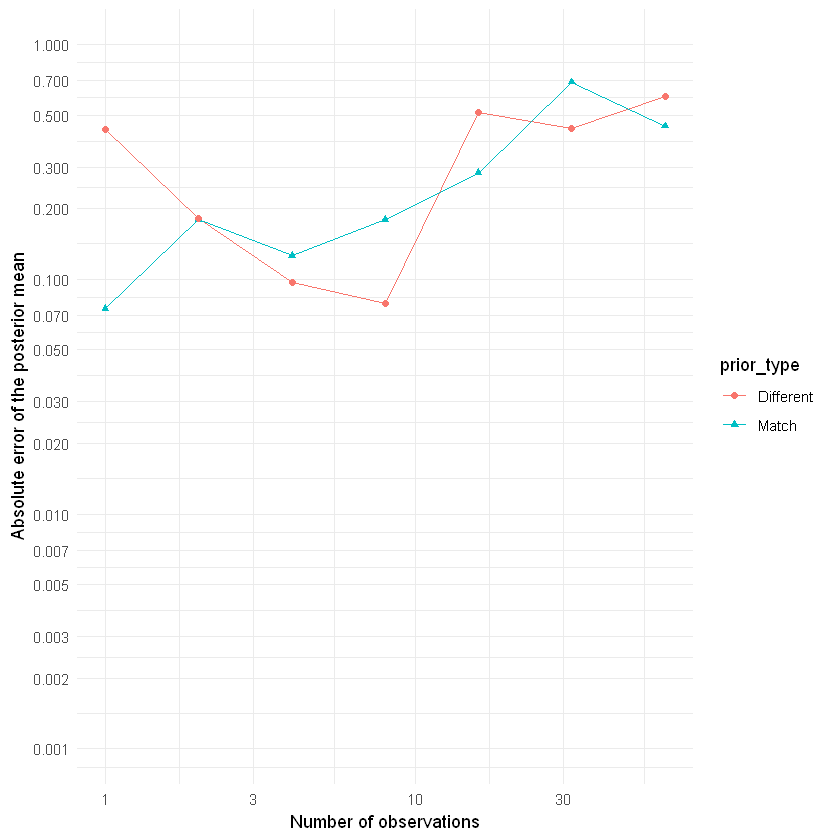
\includegraphics[width=0.9\textwidth]{two_errors.png}

From the plot above, we can see that when number of observation is small, then the error from the wrong prior is larger than from the true prior.
But as the number of observation increases, the error tends to decrease regardless of the initial choice of prior. In addition, the decreasing trend from the wrong prior seems to coincide with the trend from the true prior in the long term.




\end{enumerate}









% Optional: Feedback on assignment
% \qsol{Feedback on assignment}

 
\end{document}

